\begin{center}
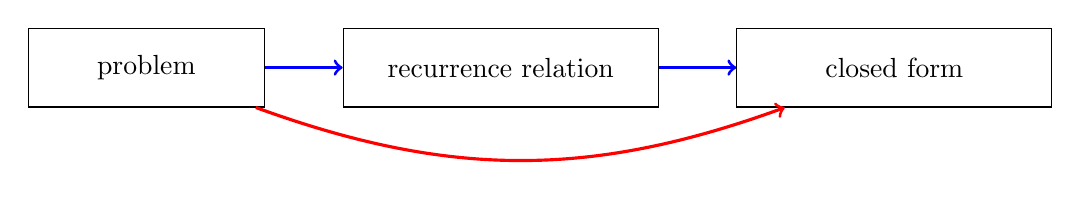
\begin{tikzpicture}

\draw (1.5, 0.5)
  node[draw, , , color=black,
       rounded corners=0cm, inner sep=0cm,
       name=problem] {

\begin{minipage}[t][1cm]{3cm}
\mbox{}

\end{minipage}

};\draw (1.5, 0.5) node[color=black] {problem};
\draw (6.0, 0.5)
  node[draw, , , color=black,
       rounded corners=0cm, inner sep=0cm,
       name=recurrence] {

\begin{minipage}[t][1cm]{4cm}
\mbox{}

\end{minipage}

};\draw (6.0, 0.5) node[color=black] {recurrence relation};
\draw (11.0, 0.5)
  node[draw, , , color=black,
       rounded corners=0cm, inner sep=0cm,
       name=closed form] {

\begin{minipage}[t][1cm]{4cm}
\mbox{}

\end{minipage}

};\draw (11.0, 0.5) node[color=black] {closed form};\draw[line width=0.04cm,blue,->] (problem) to  (recurrence);
\draw[line width=0.04cm,blue,->] (recurrence) to  (closed form);
\draw[line width=0.04cm,red,->] (problem) to [bend right=20]  (closed form);
\end{tikzpicture}

\end{center}

